\documentclass[main.tex]{subfiles}


\begin{document}

\chapter{Experimentation}
In this chapter we will Give more details about the Experiences done for reproduction
\section{Datasets}
\begin{itemize}
    \item \textbf{DSB18} : 670 images of fluorescence , bright field images of nuclei
    \item \textbf{CISD} : 3700 images of overlapping stained cells.
\end{itemize}

\begin{figure}[H]
    \centering
    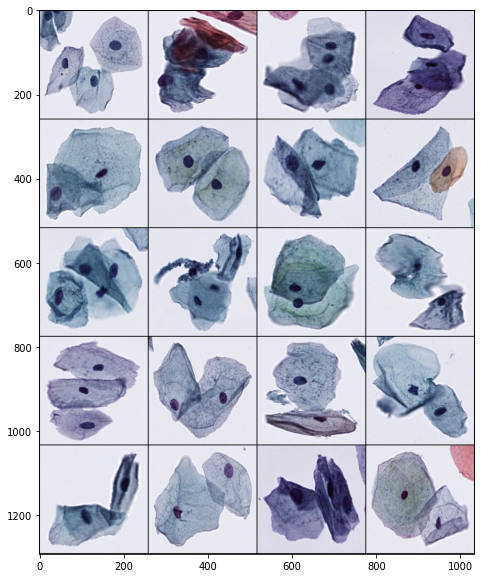
\includegraphics[width=8cm]{images/CISD.png}
    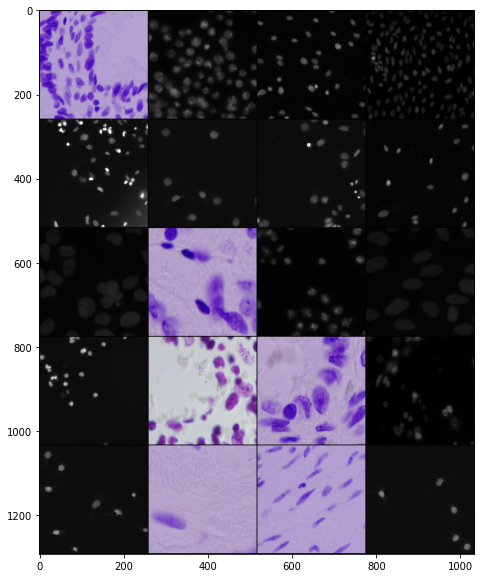
\includegraphics[width=8cm]{images/DSB18.png}
    \caption{Samples of the used datasets (CISD and DSB respectively)}
\end{figure}

\section{Training details}


\subsection{Hyperparameters choice}
We experimented with different parameters (as grid search was expensive to realize, especially due to the lack of gpus). Given the nature of the DSB dataset, the nuclei have rather elliptical shapes, so we picked a small number of control points 6, and we didn't observe any benefit from using a higher number As an educated guess, we picked a learning rate of 0.003 for Adam optimizer with an exponential decay learning rate. We use a weighted loss (as images contains more background pixels than instances pixels) we use a value of 0.2. Lambda1 is the contour loss parameter, we observed that when it's very high the probability branch takes longer to converge, so we picked a value 0.9, lambda2 is a regularization parameter for zero pixels, we picked 0.004 as used by the main article. We used object proba 0.4 as it yielded the best precision recall value in our experiments. Nms IoU threshold of 0.1 as the data didn't contain overlapping cells, otherwise we pick a higher value. For the Conv2d layers we have experimented with different kernel sizes, we saw that kernel 1 was the one that achieved the best results. we use a maximum contour length of 291 as found in the dataset. we train our network with a batch size of 4 for 400 epochs.


\subsection{Hardware and Training time}
In our experiments, we used a machine with an intel Xeon 32 cores, and an Nvidia V100 32GB RAM. Our model took 8 Hours to train (with several debug procedures activated), it should take less time when these procedures are off.

\begin{figure}[H]
    \centering
    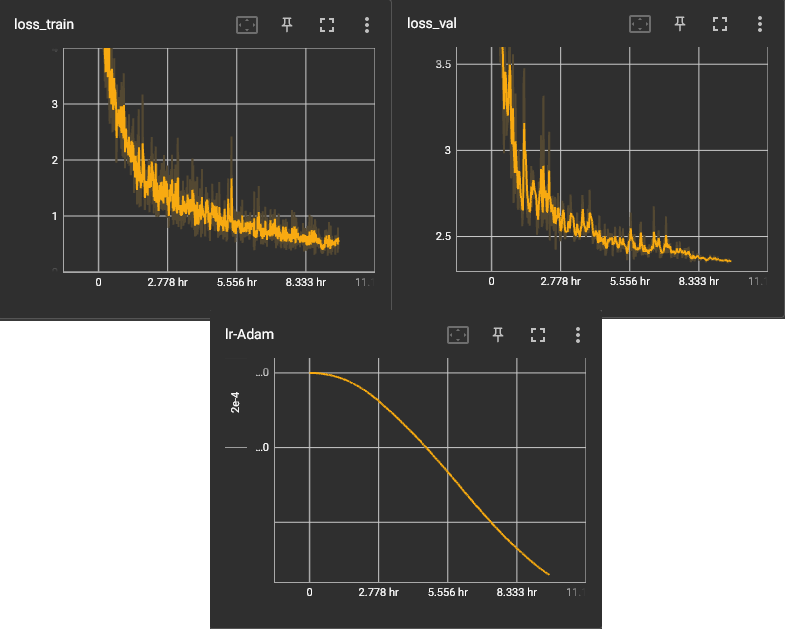
\includegraphics[width=15cm]{presentationImages/Loss.png}
    \caption{Training details}
\end{figure}

\section{Results}
We used 80\% of the data for the train and 10\% for the validation and 10 for the test.

As we can see in the predicted probabilities, the model detects very well the instances. The predicted shapes (on different sized and orientation) are well fit. some instances are not present in the right image, but are in the left one, this is due to the threshold value, and Nms threshold which were not exactly optimal. by further optimizing these parameters, we obtain better results.

\begin{figure}[H]
    \centering
    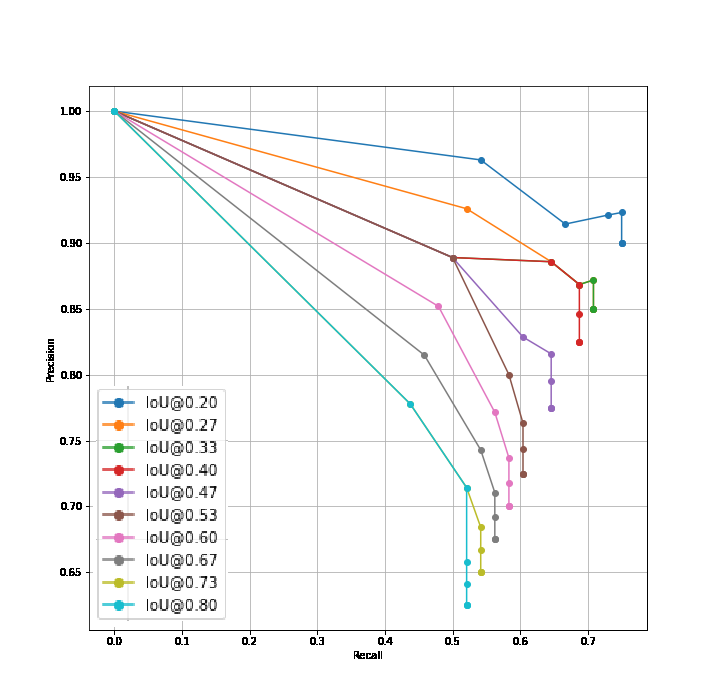
\includegraphics[width=8cm]{presentationImages/averageprecision.png}
    \caption{Average precision curve}
\end{figure}

\begin{figure}[H]
    \centering
    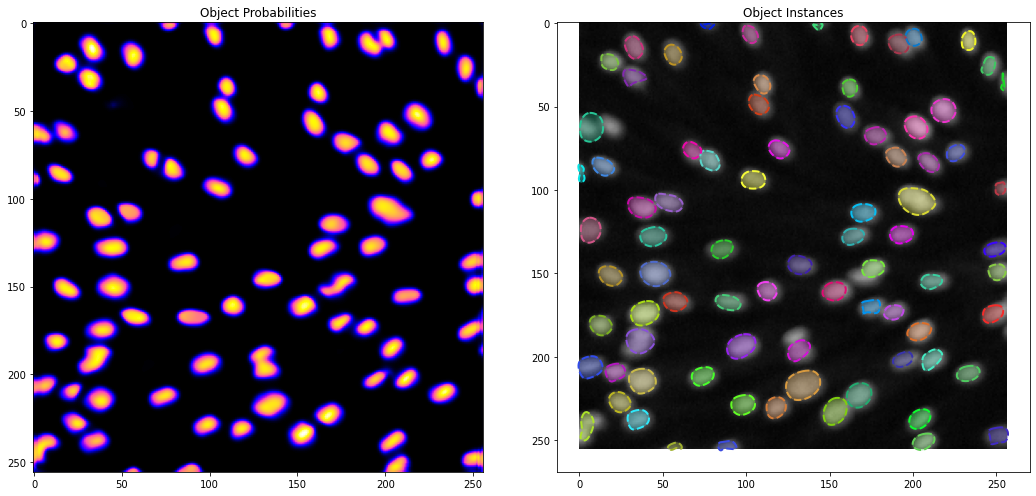
\includegraphics[width=10cm]{presentationImages/output_13_167.png}
\end{figure}

\begin{figure}[H]
    \centering
    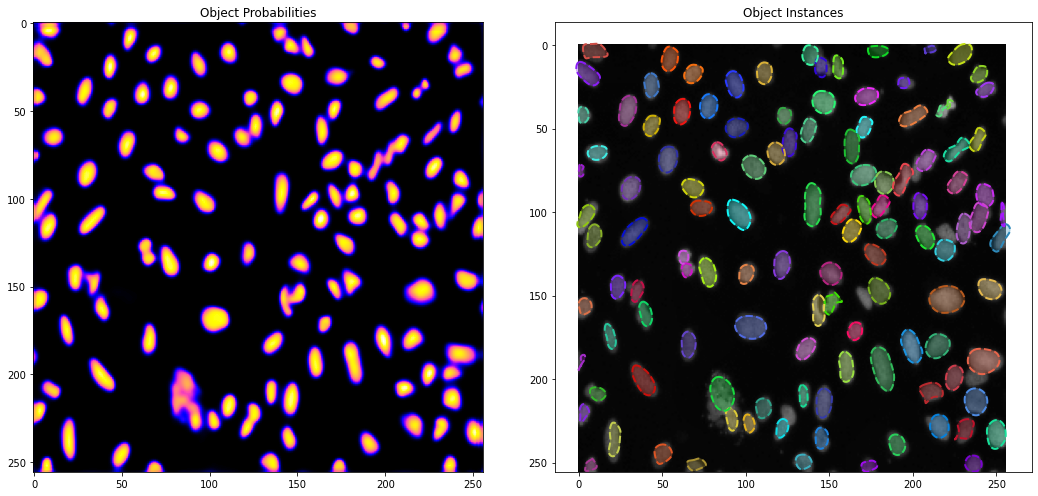
\includegraphics[width=10cm]{presentationImages/output_13_251.png}
\end{figure}

\begin{figure}[H]
    \centering
    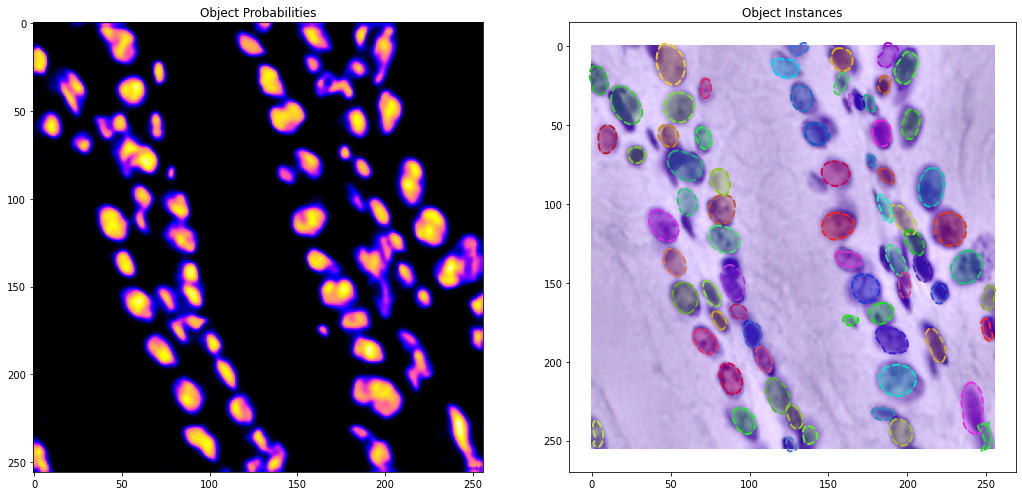
\includegraphics[width=10cm]{presentationImages/output_13_255.png}
    \caption{Results obtained using The proposed model on DSB18}
\end{figure}






\begin{figure}[H]
    \centering
    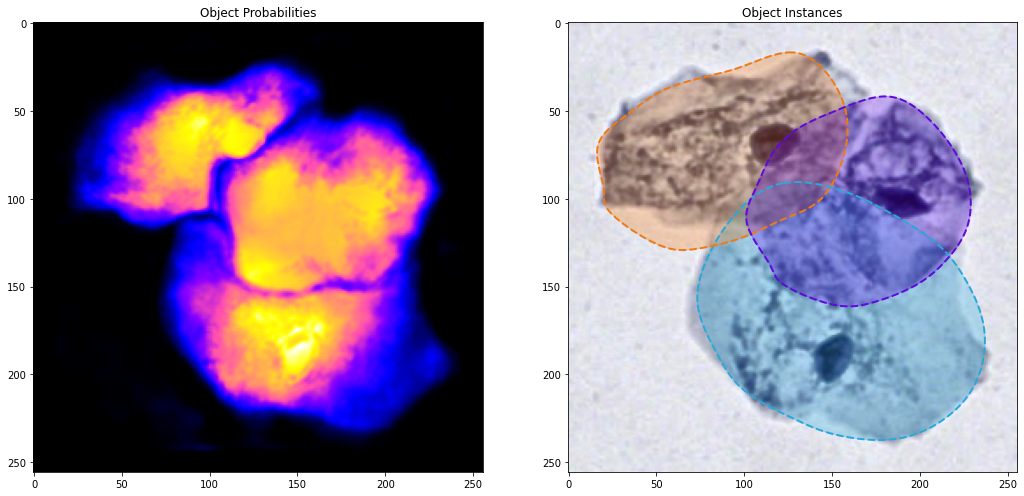
\includegraphics[width=10cm]{images/CISD_result1.png}
    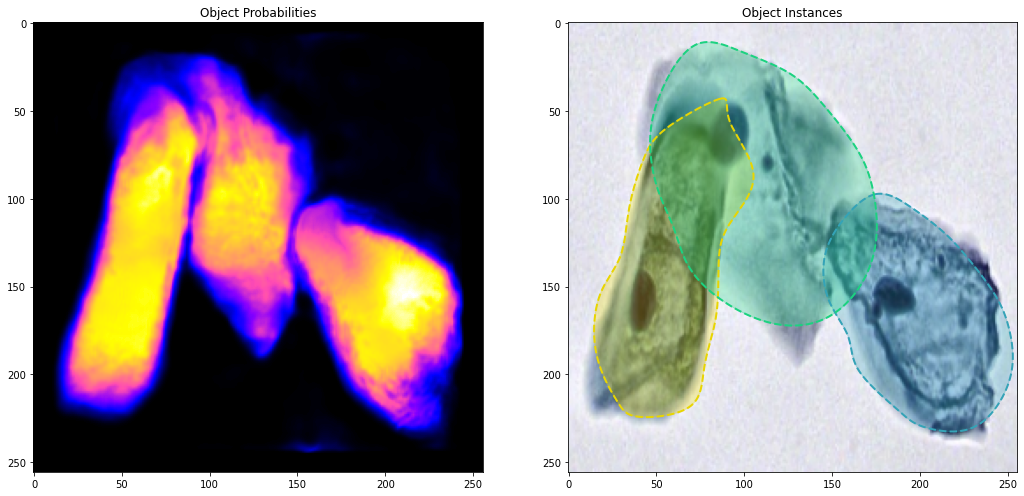
\includegraphics[width=10cm]{images/CISD_result2.png}
    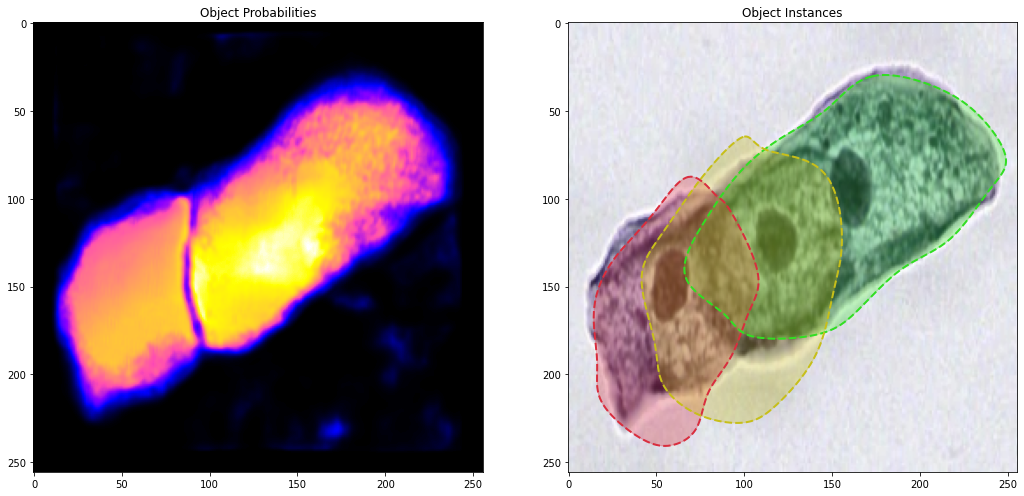
\includegraphics[width=10cm]{images/CISD_result3.png}
    \caption{Results obtained using The proposed model on CISD dataset with 16 control points and 50 epochs}
\end{figure}

\end{document}